\documentclass[fleqn, a4paper]{report}
\usepackage[top=1.5in,bottom=1.5in,left=1.15in,right=1.15in]{geometry}
\usepackage{graphicx}
\usepackage{tikz}
\usetikzlibrary{automata, positioning, arrows}
\usepackage[export]{adjustbox}
\usepackage{float}
\usepackage{gensymb}
\usepackage{amsmath}
\usepackage{booktabs}
\usepackage{tabularx}
\usepackage{lipsum}
\usepackage{pgfplots}
\usepackage{subfig}
\pgfplotsset{compat=1.15}
\usepackage[utf8]{inputenc}
\usepackage{hyperref}
\hypersetup{
    colorlinks=true,
    linkcolor=blue,
    filecolor=magenta,      
    urlcolor=cyan,
}

\title{EE463 Static Power Conversion I 
-Simulation Project II}
\author{Nail Tosun, Ozan Can İyiyer}
\date{November 2018}

\usepackage{natbib}
\usepackage{graphicx}

\begin{document}


\maketitle

\section*{Introduction}
In this simulation project, we investigated single phase and three phase controlled rectifier topologies. The differences, pros and cons of fully controlled and hald controlled single phase rectifier topologies discussed Q1. First part of the Q2 we used 3 phase full wave rectifier for driving DC motor. The speed, torque and armature current of rectifier investigated. We propose 2 methods for improving torque ripple. Then, the efficiency and components of power losses showed. Selection of diode and rectifier module be explained part 2. At Q3 we examined an alternative rectifier topology, 12 pulse rectifier, describe its operation and application areas and we showed the differences between full wave diode rectifier. 
\section*{Abbreviations}
\begin{table}[H]
\begin{tabular}{ll}
\textbf{THD} & Total Harmonic Distortion \\
\textbf{Qx}  & x'th question \\
\textbf{FFT} & Fast Fourier Transform
\textbf{PCC} & Point of Common Coupling \\
\textbf{l-l} & Line to Line \\
\textbf{pf} & Power Factor \\
\textbf{RMS} & Root Mean Square
\end{tabular}
\end{table}
\section*{Question 1}
\subsection*{Part a}
\subsubsection*{Single Phase Fully Controlled Rectifier}
Analytical calculations are following;
$$ \frac{1}{T}\int_{\alpha}^{\pi+\alpha}v_d dt = \frac{r_d}{T}\int_{\alpha}^{\pi+\alpha}i_d dt + \frac{L_d}{T}\int_{I_d(\alpha)}^{I_d(\pi+\alpha)}di_d $$
In the steady state waveforms with time period T, $I_d(\alpha)=I_d(\pi+\alpha)$ then we can say;
$$v_d = r_d I_d = 160 V$$
$$v_d = \frac{1}{\pi}\int_{\alpha+u}^{\pi+\alpha}230\sqrt{2}sin(\omega t)d\omega t=160V$$
$$cos(\alpha+u)-cos(\alpha+\pi)=1.545$$
$$cos(\alpha+u)=0.772$$
$$\alpha+u=39.40 \degree$$
$$A_u=\int_{\alpha}^{u+\alpha}V_msin(\omega t)d\omega t=\omega L_s I_d$$
$$cos(\alpha)-cos(\alpha+u)=\frac{\omega L_s I_d}{V_m}$$
$$cos(\alpha)=0.772+\frac{(2\pi 50)(0.5) 10^{-3} (40)}{230\sqrt{2}}=0.7913$$
$$\alpha=37.63 \degree$$
\begin{figure}
    \centering
    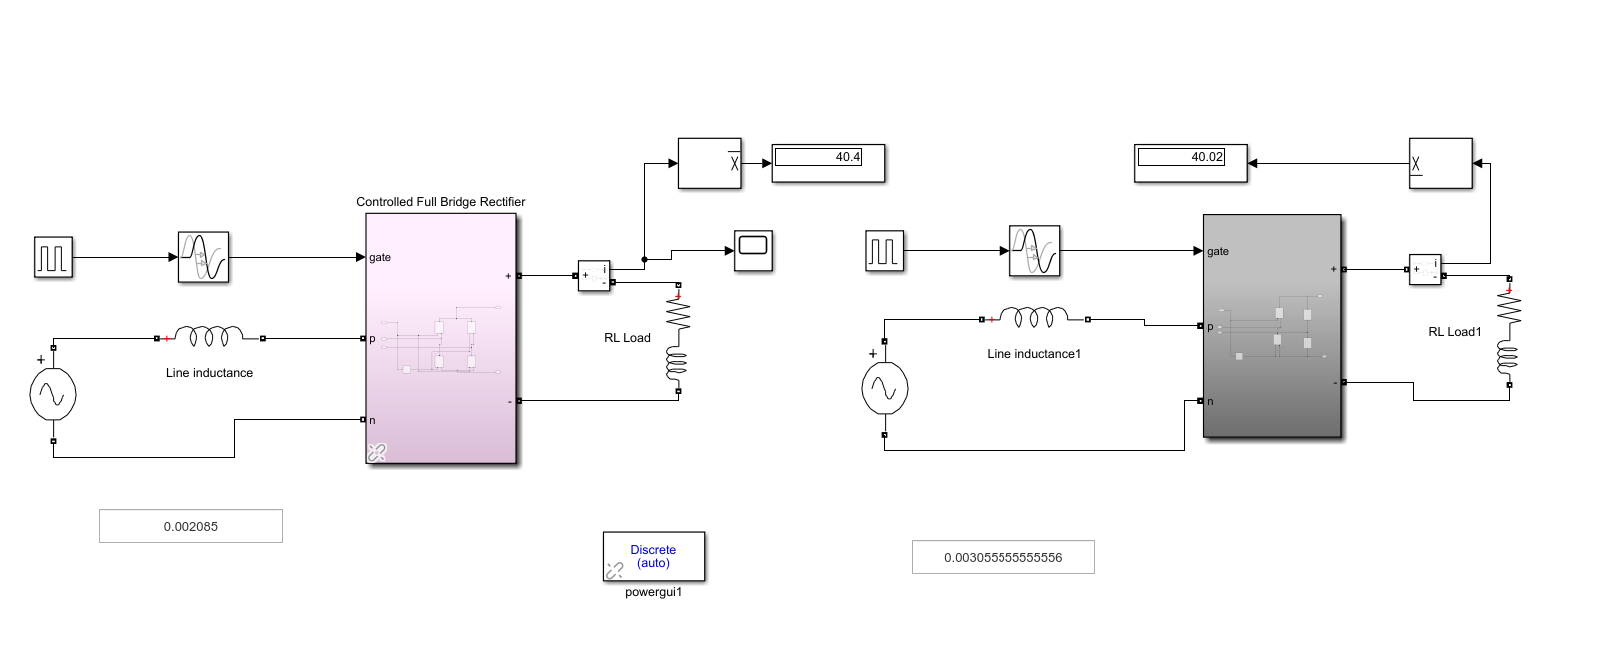
\includegraphics[width=15cm]{simulink-results.PNG}
    \caption{Simulink simulation results}
    \label{fig:my_label}
\end{figure}
\subsubsection*{Single Phase Half Controlled Rectifier}
$$v_d = \frac{1}{\pi}\int_{\alpha+u}^{\pi}230\sqrt{2}sin(\omega t)d\omega t=160V$$
$$cos(\alpha+u)-(-1)=1.545$$
$$cos(\alpha+u)=0.545$$
$$\alpha+u=56.95 \degree$$
$$A_u=\int_{\alpha}^{\alpha+u}V_m sin(\omega t)d\omega t=\omega L_s I_d$$
$$cos(\alpha)-cos(\alpha+u)=\frac{\omega L_s I_d}{V_m}$$
$$cos(\alpha)=0.545+0.0193=0.5646$$
$$\alpha = 55.625 \degree$$
\subsection*{Part b}
\begin{figure}[H]%
    \centering
    \subfloat[Fully controlled single phase rectifier]{{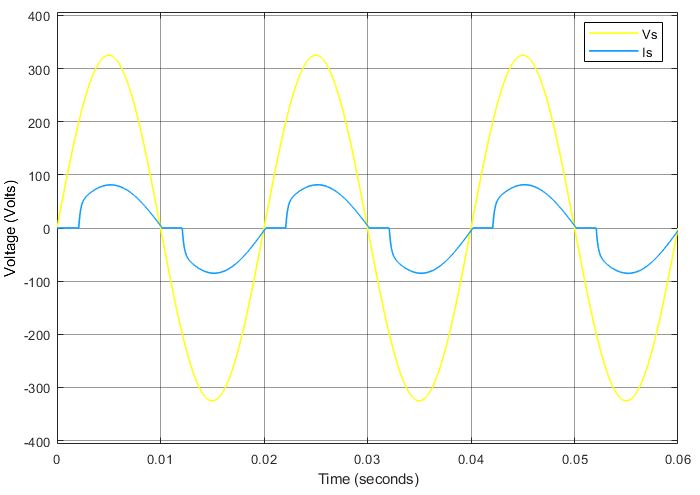
\includegraphics[width=7cm]{fullisvs.png}}}%
    \qquad
    \subfloat[Half controlled single phase rectifier]{{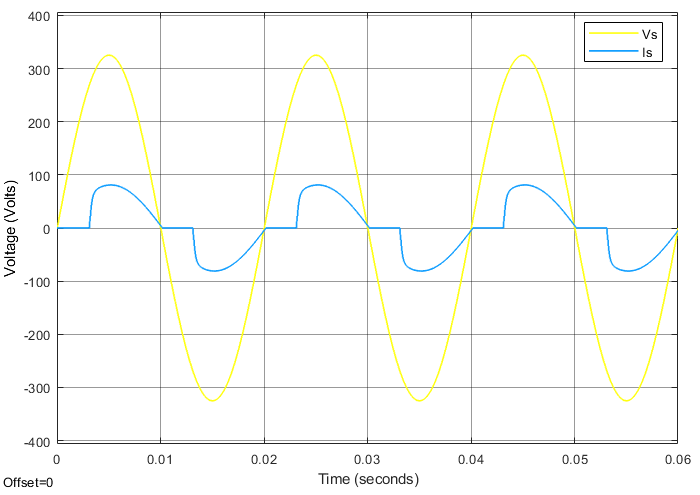
\includegraphics[width=7cm]{halfisvs.png} }}%
    \caption{Source side voltage and current waveform of both topologies}%
    \label{fig:example}%
\end{figure}
\begin{figure}[H]%
    \centering
    \subfloat[Fully controlled single phase rectifier]{{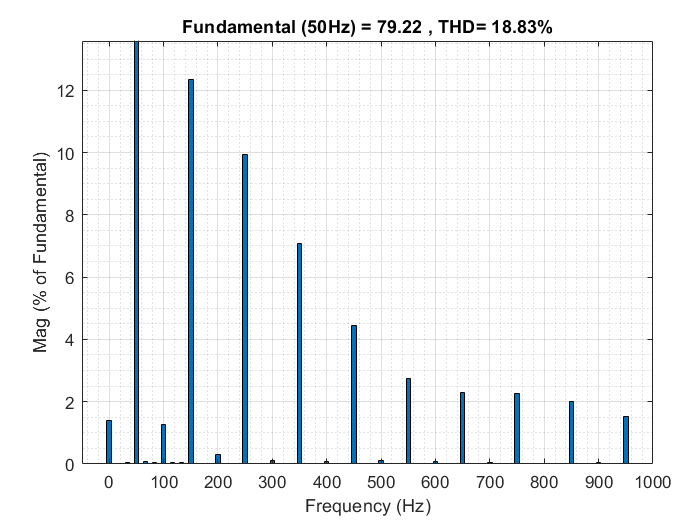
\includegraphics[width=7cm]{thdfully.png}}}%
    \qquad
    \subfloat[Half controlled single phase rectifier]{{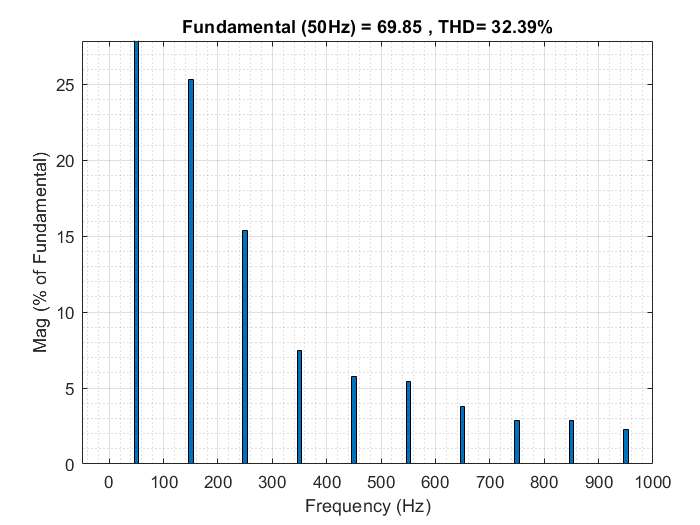
\includegraphics[width=7cm]{thdhalf.png} }}%
    \caption{Line current THD comparison of two topologies}%
    \label{fig:example}%
\end{figure}
\subsection*{Part c}
\begin{table}[H]
\begin{tabularx}{\linewidth}{>{\parskip1ex}X@{\kern4\tabcolsep}>{\parskip1ex}X}
\toprule
\hfil\bfseries Fully Controlled Rectifier
&
\hfil\bfseries Half Controlled Rectifier
\\\cmidrule(r{3\tabcolsep}){1-1}\cmidrule(l{-\tabcolsep}){2-2}

%% PROS, seperated by empty line or \par
It provide negative output voltages at output\par

It can work both rectifier and inversion modes\par

&

%% CONS, seperated by empty line or \par
It can not provide negative output voltage\par
It has less thyristors, less gate driver \par
Diodes are working as free wheeling dioded so there is no need for extra diodes

\\\bottomrule
\end{tabularx}
\caption{Comparison of half and full controlled rectifier}
\end{table}
\section*{Question 2}
\begin{figure}[H]
    \centering
    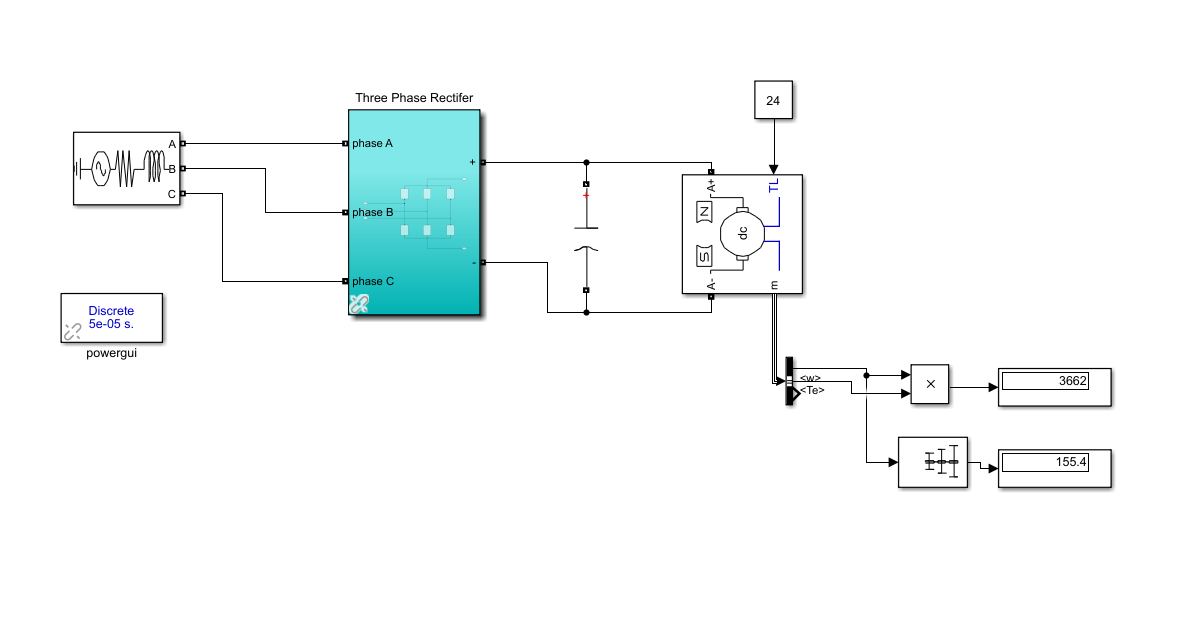
\includegraphics[width=13cm]{simulinkpart2.PNG}
    \caption{Simulink model for Q2}
    \label{fig:my_label}
\end{figure}
\subsection*{Part 1}
\begin{figure}[H]%
    \centering
    \subfloat[Armature current]{{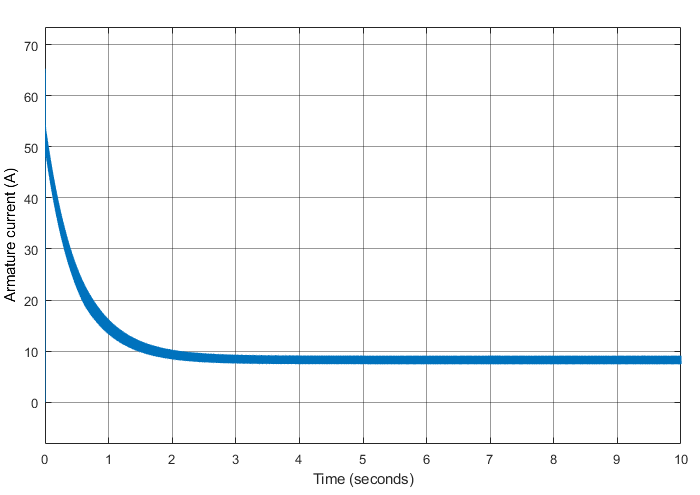
\includegraphics[width=7cm]{armature.png}}}%
    \qquad
    \subfloat[Torque]{{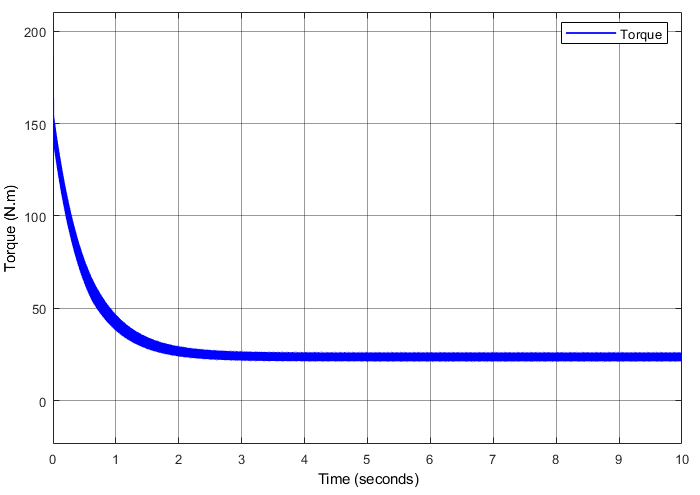
\includegraphics[width=7cm]{torque.png} }}%
    \qquad
    \subfloat[Motor Speed]{{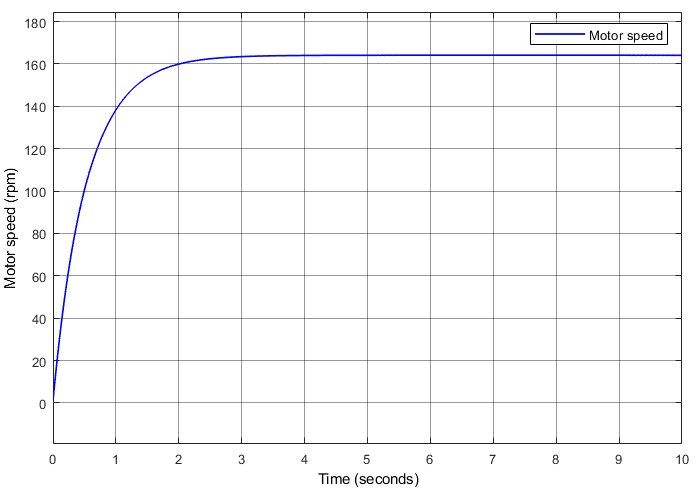
\includegraphics[width=7cm]{motorspeed.png} }}%
    \caption{DC motors output characteristics}%
    \label{fig:example}%
\end{figure}
\subsection*{Part 2}
The frequency of torque ripple is 300 Hz. The reason is that the torque of DC motor is directly related with armature current. Since the output ripple of 3 phase diode rectifier is 300 Hz and the load is simply RLC (load can not change frequency, only the magnitude and phase of the ripple can be effected by load.) armature current has same ripple frequency, 300 Hz. 
The magnitude of the torque ripple is 4.5 N.m when DC bus capacitor is 470 $\mu F$.

THD of line current is \% 144.22. When we analyze the FFT of line current, we didn't see any third harmonics components (3rd,9th..) since we have balanced three phase system. 
\begin{figure}[H]%
    \centering
    \subfloat[THD of line current]{{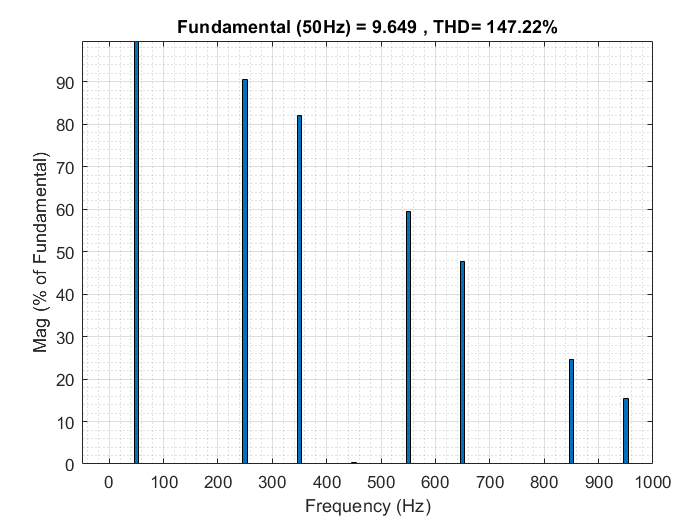
\includegraphics[width=7cm]{thdmotor.png}}}%
    \qquad
    \subfloat[Torque ripple at steady state]{{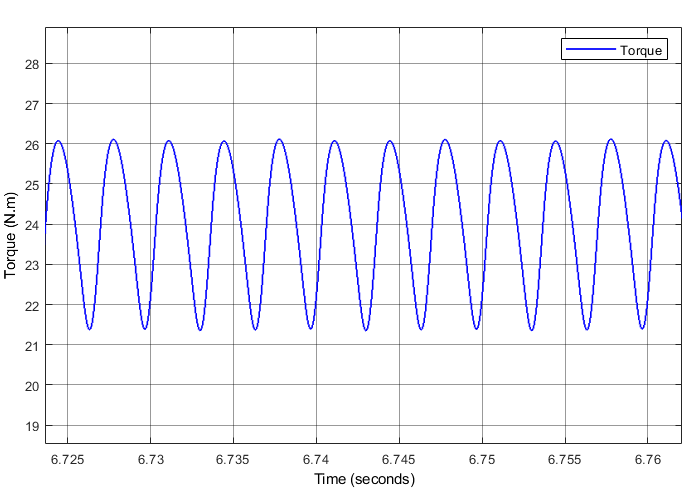
\includegraphics[width=7cm]{torqueripple.png} }}%
    \caption{THD of line current and torque ripple at the output}%
    \label{fig:example}%
\end{figure}
\subsection*{Part 3}
\subsubsection*{Adding line inductor armature side}
\begin{figure}[H]%
    \centering
    \subfloat[Torque]{{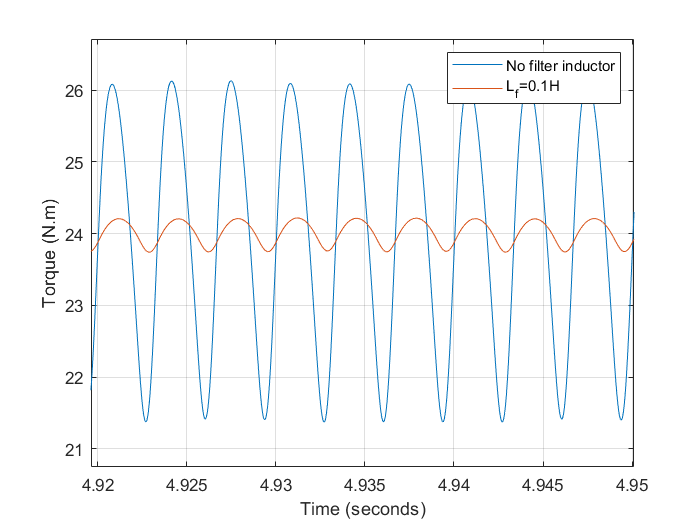
\includegraphics[width=7cm]{addinginductancetorque.png}}}%
    \qquad
    \subfloat[Armature current]{{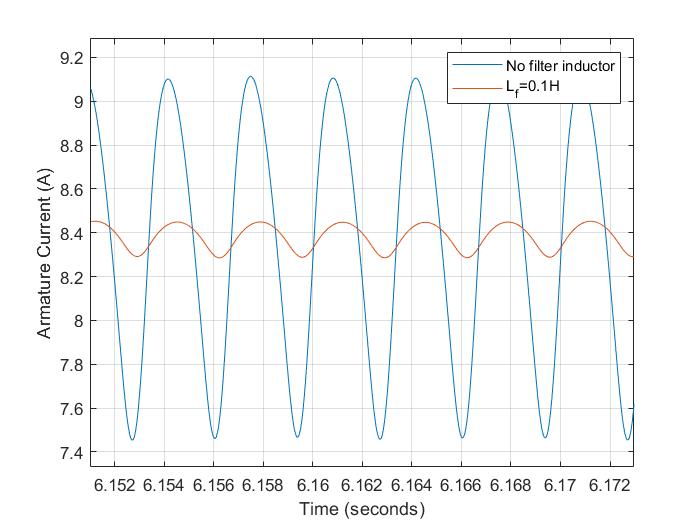
\includegraphics[width=7cm]{addinginductancearmature.png}} }%
    \caption{The effect of adding filter inductor to armature side}%
    \label{fig:example}%
\end{figure}
\subsubsection*{Improving DC bus capacitor}

\begin{figure}[H]%
    \centering
    \subfloat[THD of line current]{{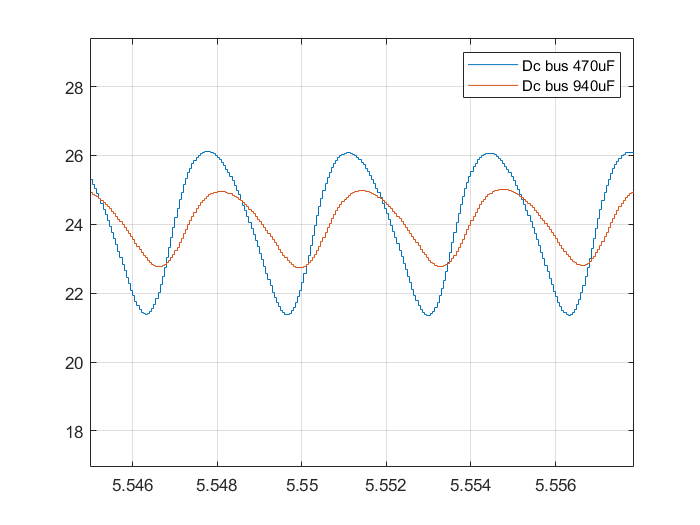
\includegraphics[width=7cm]{dcbus.png}}}%
    \qquad
    \subfloat[Torque ripple at steady state]{{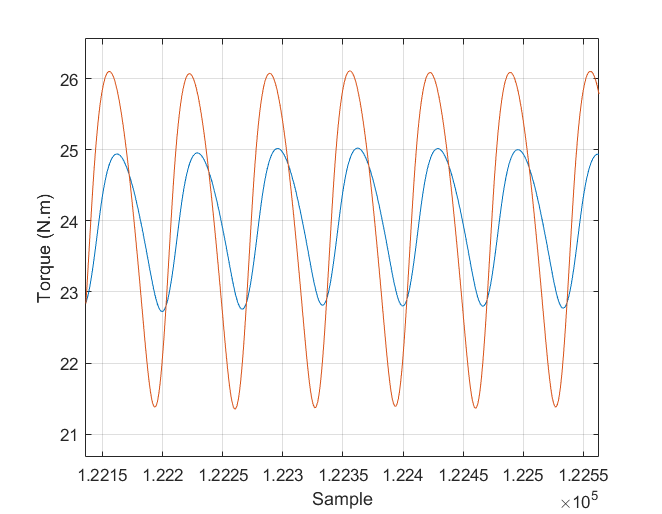
\includegraphics[width=7cm]{dcbuss.png} }}%
    \caption{THD of line current and torque ripple at the output}%
    \label{fig:example}%
\end{figure}
\begin{table}[H]
\begin{tabularx}{\linewidth}{>{\parskip1ex}X@{\kern4\tabcolsep}>{\parskip1ex}X}
\toprule
\hfil\bfseries Pros
&
\hfil\bfseries Cons
\\\cmidrule(r{3\tabcolsep}){1-1}\cmidrule(l{-\tabcolsep}){2-2}

%% PROS, seperated by empty line or \par
It significantly reduce armature current ripple, thus torque ripple\par

More robust when we think closed loop system control as alternative\par

&

%% CONS, seperated by empty line or \par
Bulky inductor and DC bus capacitor increases driver volume drastically. \par
Power density of driver decreased \par

\\\bottomrule
\end{tabularx}
\caption{Pros and Cons of adding passive filtering elements to the output}
\end{table}

\subsection*{Part 4}
$$\eta = \frac{P_{mech}}{P_{elec}}=\frac{T \omega}{3 V_{rms} I_{rms} pf} = \frac{3939.36}{4692} = 0.8395 $$
\subsubsection*{Cupper losses}
Cupper losses can happen on armature resistance,$r_a$ ,source resistance,$r_s$ or diode on resistance,$r_{on}$. Passive elements like capacitors and inductors have also parasitic resistance components, but since we didn't model them in simulation we didn't calculate their losses. 
$$P_{r_a}=I_a_{rms}^2 r_a=716.22 \>W$$
$$P_{r_{on}}=6 I_d_{rms}^2 r_{on} = 8.76 \>W$$
$$P_{r_s}=3 I_s_{rms}^2 r_s = 44.286 \> W$$

\subsubsection*{Switching losses}
Since the voltage and current of practical diode can not be change instantly there is a switching loss when continuously opening and closing the diode. To find switching loss we look at three phase diode rectifier as black box. We look at input and output power flow. The difference is indicating switching loss and $r_{on}$ cupper loss. Since we know cupper loss it is easy to execute switching loss. 
$$P_{sw} = 10.38 W$$
\subsubsection*{Mechanical losses}
When we calculating overall efficiency, we also look at mechanical losses like friction. However, we didn't model viscous friction at DC Machine model (B = 0 N.m.s).Therefore, there is no mechanical loss in this model. 
\begin{figure}[H]
    \centering
    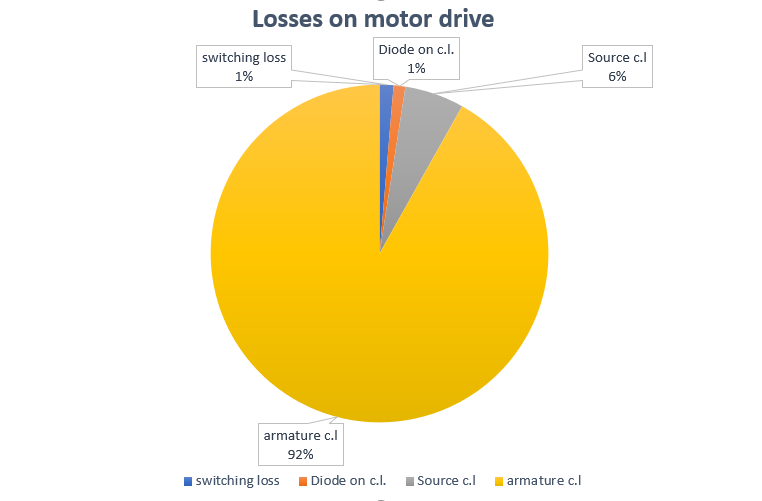
\includegraphics[width=10cm]{losses.PNG}
    \caption{Losses in pie chart}
    \label{fig:my_label}
\end{figure}




\section*{Question 3}
\subsection*{Part a}
The topology which indicated at Figure 9.a is named as Twelve Pulse Rectifier. The circuit mainly takes 3 phase voltage input and rectifies it to 12 pulse DC signal over one period with the help of two 6 phase bridge rectifiers. The purpose of using one primary and two secondary transformers is obtaining 300 phase shifted voltage output at secondary side. Therefore, 5th and 7th harmonics will be eliminated and THD will be reduced.

The other CCT topologies which can be used for similar purpose are Half-wave 12-pulse rectifier (single-way) and 12-pulse bridge rectifier (parallel connection) which can be seen from Figure 9.b and Figure 9.c. Unlike other topologies, at Half-wave 12-pulse rectifier we connect 12 phases via interconnection transformers. In series connection rectifier we provide centre point for earthing purposes. As a final note we can say that because of their special transformer needs 12 pulse rectifiers are very expensive devices.
\begin{figure}[H]%
    \centering
    \subfloat[12 pulse rectifier series connection(1)]{{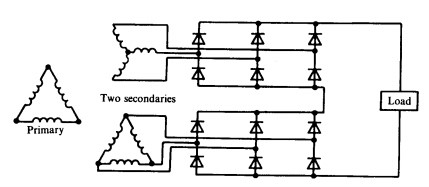
\includegraphics[width=7cm]{one.jpg}}}%
    \qquad
    \subfloat[Half wave 12 pulse rectifier(2)]{{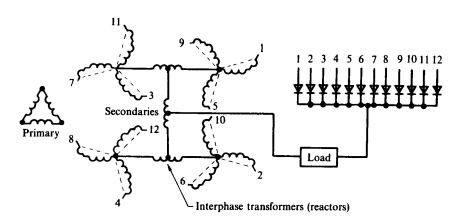
\includegraphics[width=7cm]{second.png} }}%
    \qquad
    \subfloat[12 pulse rectifier parallel connection(3)]{{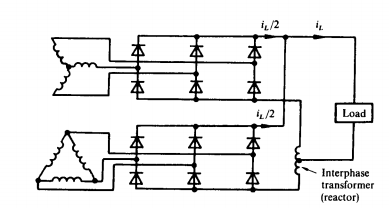
\includegraphics[width=7cm]{third.png} }}%
    \caption{Different 12 pulse rectifier topologies}%
    \label{fig:example}%
\end{figure}

\subsection*{Part b}
We have simulated both Twelve Pulse Rectifier (can be seen from Figure) and Full Bridge Rectifier for same average output voltage values. The simulation results indicated at Figures 5 and 6. According to the findings, we observed that the ripple voltage decreased for 12 Pulse Rectifier. Because our load is purely resistive the same situation is valid for output load currents. In addition, we can say that the cost of twelve pulse rectifier construction will be more expensive because of delta-delta-wye connected transformers. The maximum output voltage and current -and hence RMS values- is higher for Full Bridge Rectifier.

\begin{figure}[H]%
    \centering
    \subfloat[Simulink diagram]{{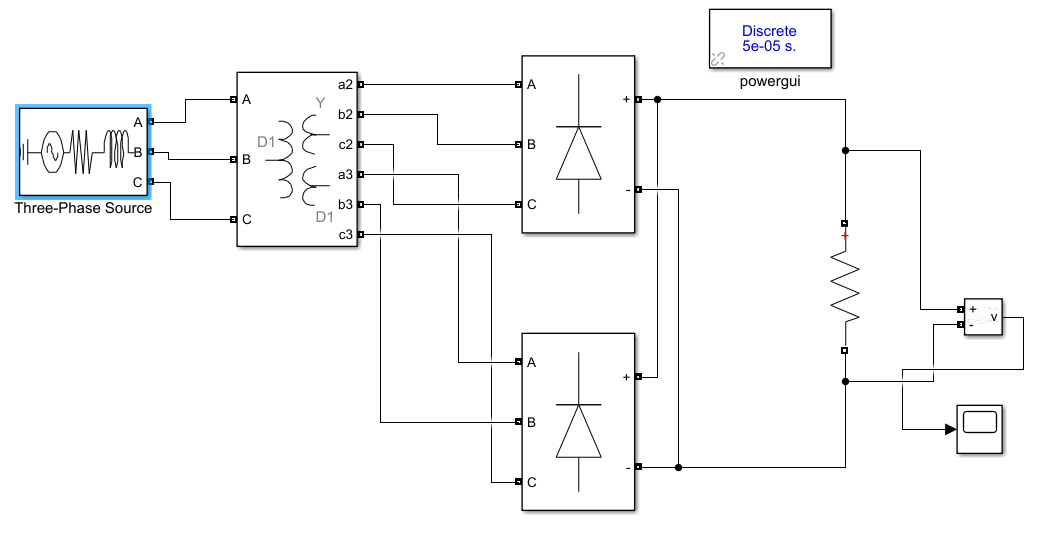
\includegraphics[width=7cm]{fourth.png}}}%
    \qquad
    \subfloat[Simulation results]{{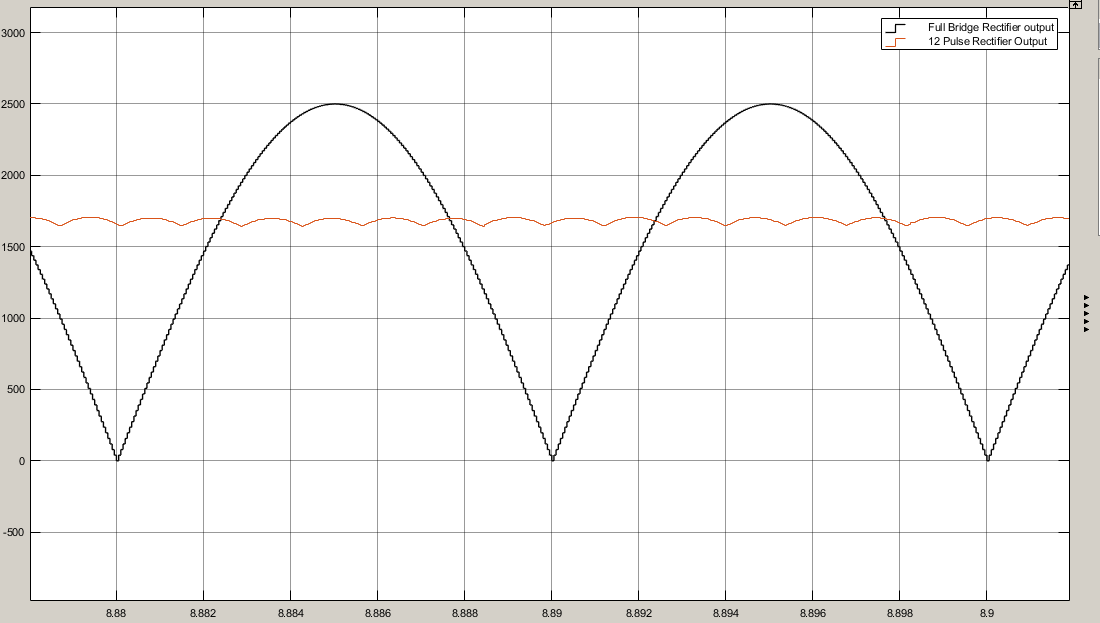
\includegraphics[width=7cm]{fifth.png} }}%
    \caption{Simulation results of 12 pulse rectifier}%
    \label{fig:example}%
\end{figure}



\subsection*{References}
[1][2][3] MOHAN, N. (2017). Power Electronics JOHN WILEY & Sons.
\end{document}
